\chapter{Materiales y métodos}\label{C:Materiales}
\graphicspath{{./figs/02_Mat/}}
\section{Experimentos de difracción de rayos X}\label{S:MatXRD}
Buena parte del trabajo de esta tesis se centró alrededor de los experimentos de difracción de rayos X.
En particular, la mediciones se hicieron empleando la geometría de transmisión, también llamada de Debye-Scherrer, utilizando radiación sincrotrón.
La facilidad en la que se trabajó fue PETRA III, cuya fotografía puede verse en la Fig. \ref{fig:desyfoto}, y está ubicada en el complejo DESY, en la ciudad de Hamburgo, Alemania\cite{desy}.

\begin{figure}[!htb] 
  \centering
  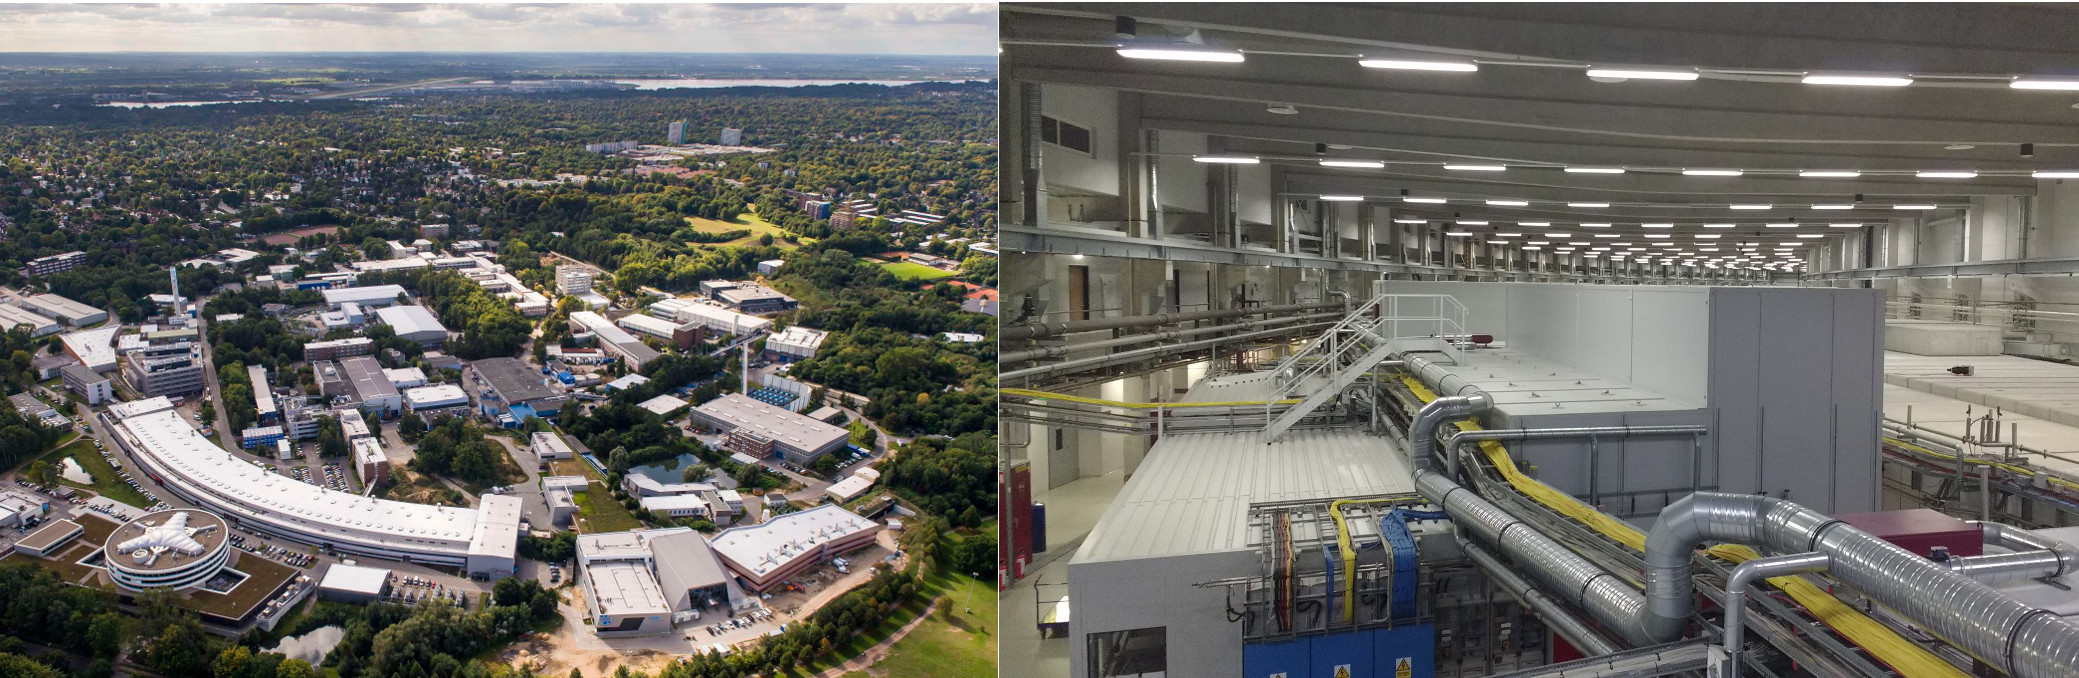
\includegraphics[width=\textwidth]{desy}
  \caption{Fotografías del exterior e interior de la facilidad PETRA III, en DESY. Imágenes obtenidas de \cite{desy}.}
  \label{fig:desyfoto}
\end{figure}

En los experimentos de transmisión realizados, se hizo incidir un haz de rayos\,X con $\lambda \ \approx \ 0.0142$\,nm sobre una muestra, como está esquematizado en la imagen de la Fig. \ref{fig:transmision}. 

Como resultado de la interacción elástica entre el haz incidente y el material, diferentes haces con la misma energía que el incidente, son dispersados por diferentes familias de planos en ángulos que están dados por la Ley de Bragg \ref{eq:Bragg}.
Para una dada familia de planos $\{hkl\}$ todos los haces difractados están comprendidos en un cono, que al interceptar el detector forman un círculo, denominado anillo de Debye, y la intensidad del haz difractado a lo largo de largo del anillo de Debye está determinada por la cantidad de planos cristalinos en condición de difracción para esa dada orientación de la muestra.

En la configuración que se muestra en la Fig. \ref{fig:transmision} la muestra se colocó en un portamuestra que permitía la alineación con el haz y el detector, y le daba a la misma la libertad de girar alrededor de un eje vertical que pasaba por su centro.
La muestra giraba gracias a un motor paso a paso y que permitía rotarla con una precisión de 5\,$^{\circ}$ por paso.
Para obtener una caracterización completa de la textura de la muestra, fue necesario rotar la misma un rango de 180\,$^{\circ}$, lo que sumado al paso de la rotación significó que por cada muestra se obtuvieron 37 anillos de Debye.

\begin{figure}[!htb]
  \centering
  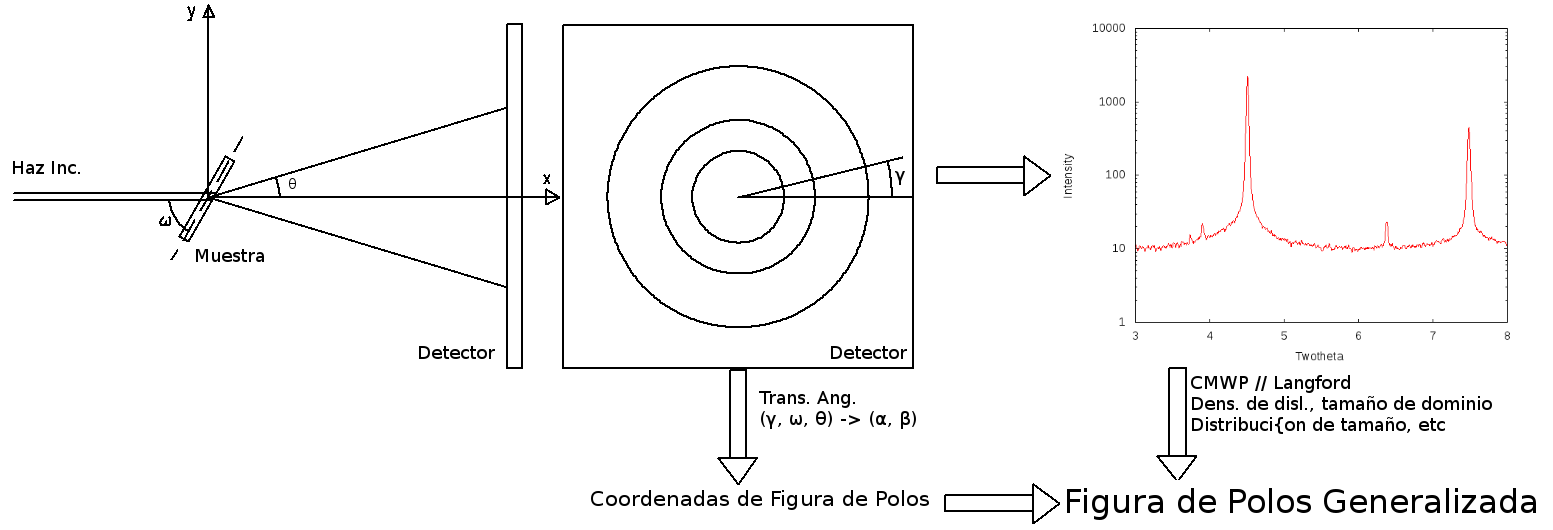
\includegraphics[width=\textwidth]{process}
  \caption{Esquema básico del proceso de medición y análisis de datos. Las mediciones se realizaron empleando una geometría de transmisión, para diferentes rotaciones $\omega$ de la muestra. Por cada posición de la muestra se registraron una serie de anillos de Debye, a partir de los cuales se extrajeron porciones radiales, con las que se construyeron difractogramas que luego fueron procesados siguiendo diferentes modelos de LPA. A partir de estos resultados, y realizando la conversión adecuada de las coordenadas de laboratorio a las coordenadas del sistema de referencia del cristal, se construyeron figuras de polos y figuras de polos generalizadas.}
  \label{fig:transmision}
\end{figure}

\nomenclature{LPA}{Análisis de ancho de pico}

El haz que incidente tenía un tamaño de 100\,$\mu$m x 100\,$\mu$m, lo que permitía obtener una gran resolución sobre la microestructura del material.
Las muestras empleadas eran varillas aproximadamente cuadradas, con su eje colocado verticalmente, es decir, paralelo al eje de giro.
El ancho de las varillas era de entre 2\,mm y 5\,mm, y se tuvo especial cuidado durante la alineación de que el haz esté completamente adentro de la muestra en todo el rango de rotación de la misma.

Se utilizó un detector de estado sólido Mar345 de forma cuadrada, con una grilla de 3450\,pixels x 3450\,pixels, de 100\,$\mu$m x 100\,$\mu$m cada uno.
El detector se colocó 1081\,mm detrás de la muestra, y los tiempos de detección se modificaron de acuerdo a la intensidad de salida del haz y la absorción de la muestra, de modo de que las intensidades máximas siempre estén cerca del número máximo de cuentas adquiribles por el detector.

De cada medición se extrajeron 37 imágenes, cada una de las cuales contaba con conjuntos de 5 a 7 anillos de Debye, dependiendo de la muestra.
De cada imagen se extrajeron porciones radiales de ancho angular de 5\,$^{\circ}$ a partir de las cuales se construyeron 72 difractogramas.
El conjunto de 72 x 37 = 2664 difractogramas fue analizado utilizando diferentes modelos de LPA, pero hubo dos modelos sobre los que se hizo especial foco: el de Langford (Sec. \ref{SS:Langford}) y el CMWP (Sec. \ref{SS:CMWP}), y de cada modelo empleado se extrajo diferente información sobre la microestructura de la muestra.

Cada pico de cada difractograma quedaba identificado por su ángulo de Bragg $\theta_B$, su coordenada angular $\gamma$ en el anillo de Debye y la rotación de la muestra $\omega$ cuando se realizó la medición, por lo que la información microestructural que se extraía del ancho de los picos era susceptible de ser graficada empleando figuras de polos, de la misma manera que se grafican las figuras de polos.
Para construir figuras de polos a partir de las mediciones realizadas fue preciso transformar las coordenadas de los picos en el sistema de laboratorio $(\omega, \gamma, \theta_B)$ a la del sistema de referencia del cristal $(\alpha, \beta)$, para lo cual se empleó la matriz de rotación ya calculada por Bunge y Klein\cite{Bunge1996}.
La misma expresión fue empleada para generar las figuras de polos generalizadas.

\subsection{Contribuciones instrumentales al ancho de pico}\label{SS:inst}
Para poder realizar un análisis microestructural preciso a partir de mediciones de ancho de pico, es necesario dar cuenta del ancho instrumental del equipo empleado.
Se define como ancho instrumental al ensanchamiento que se observa alrededor de los picos de Bragg, y que es independiente de la microestructura de la muestra estudiada.
Para medir el ancho instrumental se emplean muestras patrones, es decir, muestras que poseen una geometría similar a la de las muestras a estudiar y que no poseen ensanchamiento (o poseen un ensanchamiento muy pequeño) debido a factores microestructurales, como ser tensiones internas y tamaño de grano.
También es necesario que los patrones instrumentales no posean ningún tipo de textura.
Para las mediciones de este trabajo se utilizó un polvo de LaB$_6$ como patrón instrumental.

En la Fig. \ref{fig:LaB6vsGamma} puede verse el ancho de uno de los picos del patrón de LaB$_6$ a lo largo del anillo de Debye para tamaños de haz de 100\,$\mu$m x 100\,$\mu$m y 500\,$\mu$m x 500\,$\mu$m.
Notar que no sólo el ancho instrumental se reduce con el tamaño del haz, sino que además existe una variación del mismo a medida que se recorre el anillo de Debye, con mínimos en 90\,$^{\circ}$ y 270\,$^{\circ}$, un máximo local en 180\,$^{\circ}$ y un máximo absoluto en 0\,$^{\circ}$/360\,$^{\circ}$, y que esta variación se reduce también con el tamaño del haz, aunque nunca desaparece del todo.

\begin{figure}[!htb]
  \centering
  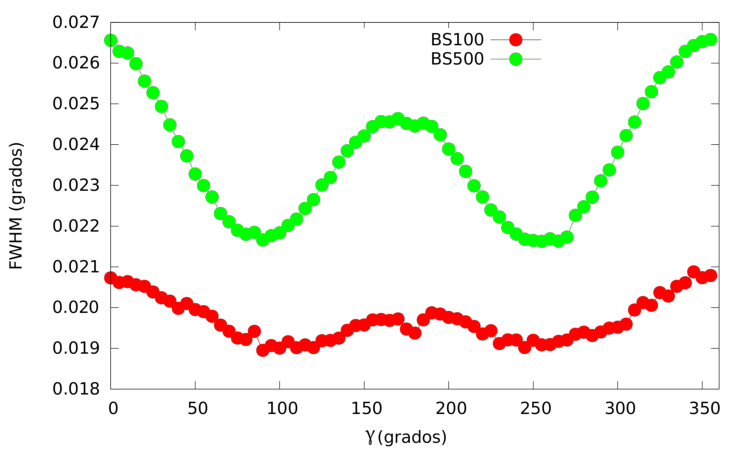
\includegraphics[width=0.95\textwidth]{LaB6_1mm_FWHMvsGammavsBS.pdf}
  \caption{Variación del ancho instrumental como función del ángulo $\gamma$ a lo largo del anillo de Debye para diferentes tamaños del haz incidente. Puede apreciarse que reducir el tamaño del haz reduce el valor promedio del ancho instrumental. También puede verse que el ancho instrumental no es uniforme a lo largo de todo el anillo de Debye, sino que se presentan oscilaciones que también se reducen al reducir el área del haz incidente.}
  \label{fig:LaB6vsGamma}
\end{figure}

La razón de esta oscilación en el ancho instrumental se debe a la divergencia del haz de rayos X\cite{Wcislak2002} y esta es una fuente de errores sistemáticos bastante común en los experimentos realizados con geometrías de transmisión, aunque su presencia suele quedar enmascarada cuando el ensanchamiento de los picos debido a la microestructura es mucho más grande que el instrumental.

En casos donde el ensanchamiento de la muestra no es tan grande, la contribución de la divergencia del haz se puede apreciar fundamentalmente como una asimetría izquierda-derecha en las figuras de polos generalizadas de ancho de pico, en el que el lado derecho e izquierdo tienen la misma estructura general, pero el derecho tiene un valor promedio visiblemente más alto, como se ve en la Fig. \ref{fig:IF75NoSym}-a.

\begin{figure}[!htb] 
  \centering
  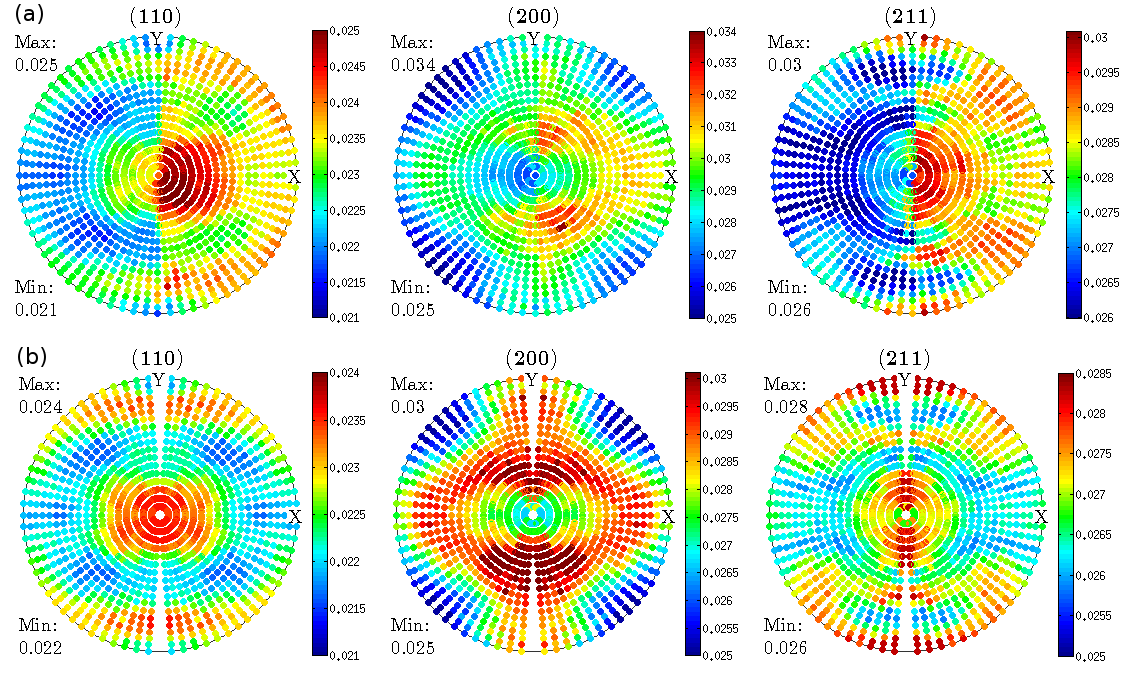
\includegraphics[width=0.95\textwidth]{IF75_SymnoSym}
  \caption{Efecto de la contribución de la divergencia del haz al ancho de pico medido. En la parte (a) de la figura pueden observarse las figuras de polos generalizadas de ancho de pico de una muestra de acero libre de instersticiales. Se observa que los datos a la derecha tienen una estructura similar a la de los de la izquierda, sólo que con un valor medio un poco más alto. En la parte (b) de la figura se simetrizó la figura de polos a partir de reflejar los datos de la izquierda a la derecha.}
  \label{fig:IF75NoSym}
\end{figure}

Inicialmente se intentó hacer una sustracción del ancho instrumental a partir de ajustar el patrón de LaB$_6$ y ajustar la componente lorentziana y gaussiana de cada uno de los picos empleando la expresión de Caglioti\cite{Caglioti1958}, para luego restar el ancho instrumental al medido en los experimentos:
\begin{align}
  H_L^{micr} & = H_L^{exp} \ - \ H_L^{inst} \nonumber \\
  (H_G^{micr})^2 & = (H_G^{exp})^2 \ - \ (H_G^{inst})^2 
  \label{eq:instrumental}
\end{align}
\noindent
donde $H_i^{micr}$, $H_i^{exp}$ y $H_i^{inst}$ representan los ensanchamientos microestructurales, experimentales e instrumentales respectivamente, y la substracción que se hace es la que corresponde atendiendo al carácter lorentziano o gaussiano de los picos.

Para hacer sustracción se decidió integrar la intensidad a lo largo de todos los anillos, y emplear este difractograma ''promedio'' para hacer los ajustes de los que se obtendrían los valores $H_L^{inst}$ y $H_G^{inst}$  que se emplearían en las Ecs. \ref{eq:instrumental}.
El problema que se manifestó al tratar el ensanchamiento instrumental de esta manera fue que las oscilaciones observadas en la Fig. \ref{fig:LaB6vsGamma}, aunque pequeñas representan una parte no despreciable de los ensanchamientos medidos.
El otro problema que se observó es que como los ensanchamientos medidos son muy pequeños, al restar los anchos instrumentales, lo valores resultantes de $H_L^{micr}$ y $H_G^{micr}$ resultaban tener un error mucho mayor que el que era razonable esperar a partir de los datos obtenidos.

Fue por estas razones que se decidió no restar el ancho instrumental cuando se realizaran análisis empleando el método de Langford, y teniendo en cuenta que todos los procesos mecánicos producen texturas con simetría ortorrómbica, se procedió a realizar los análisis empleando sólo la mitad izquierda de las figuras de polos generalizadas.
Para facilitar el análisis y observación de las FPG se decidió simetrizar las mismas, como se muestra en la Fig. \ref{fig:IF75NoSym}-b y emplear dichas figuras simetrizadas para el cálculo de las FDOG, y dado que el método de Langford y de las FPOG son métodos semi-cuantitativos para empezar, se considera que no se está perdiendo generalidad ni validez en los análisis al no restar la contribución instrumental al ancho de pico.

Por otro lado, teniendo en cuenta la geometría y simetría de los materiales estudiados, y que las oscilaciones tienen su mínima amplitud en el rango de 90\,$^{\circ}$ a 270\,$^{\circ}$, la contribución instrumental se puede considerar como un aporte constante e igual para todas las FPGs analizadas, lo que permitió realizar afirmaciones certeras acerca de los \textit{cambios} en la microestructura, por más que no se puedan hacer afirmaciones sobre los valores absolutos que determinan la misma con el mismo nivel de certeza.

\subsection{Postprocesamiento de los datos}\label{SS:MatPost}
Para poder medir la textura y realizar los estudios de ancho de pico, fue necessario procesar las imágenes obtenidas del detector de estado sólido, para extraer la información de las intensidades en forma de difractogramas. 
Las intensidades fueron escritas en archivos de texto de modo tal que la información numérica pueda ser procesada por programas de computadora.

Las imágenes obtenidas por el detector Mar345 fueron procesadas con el programa FIT2D\cite{FIT2D}, que permitió obtener porciones radiales con $\Delta \gamma \ = \ 5\,^{\circ}$ de ancho para cada conjunto de anillos, permitiendo obtener un difractograma para cada porción radial en la imagen registrada, como se muestra en la Fig. \ref{fig:fit2d}.
Como cada anillo comprende un ángulo de 360\,$^{\circ}$, para cada uno de los 37 ángulos $\omega$ que representa el giro de la muestra, se obtuvieron 72 difractogramas, cada uno de los cuales tenía asociado el par de coordenadas $(\omega, \gamma)$, que marcaba su posición angular en el sistema de laboratorio.

\begin{figure}[!htb] 
  \centering
  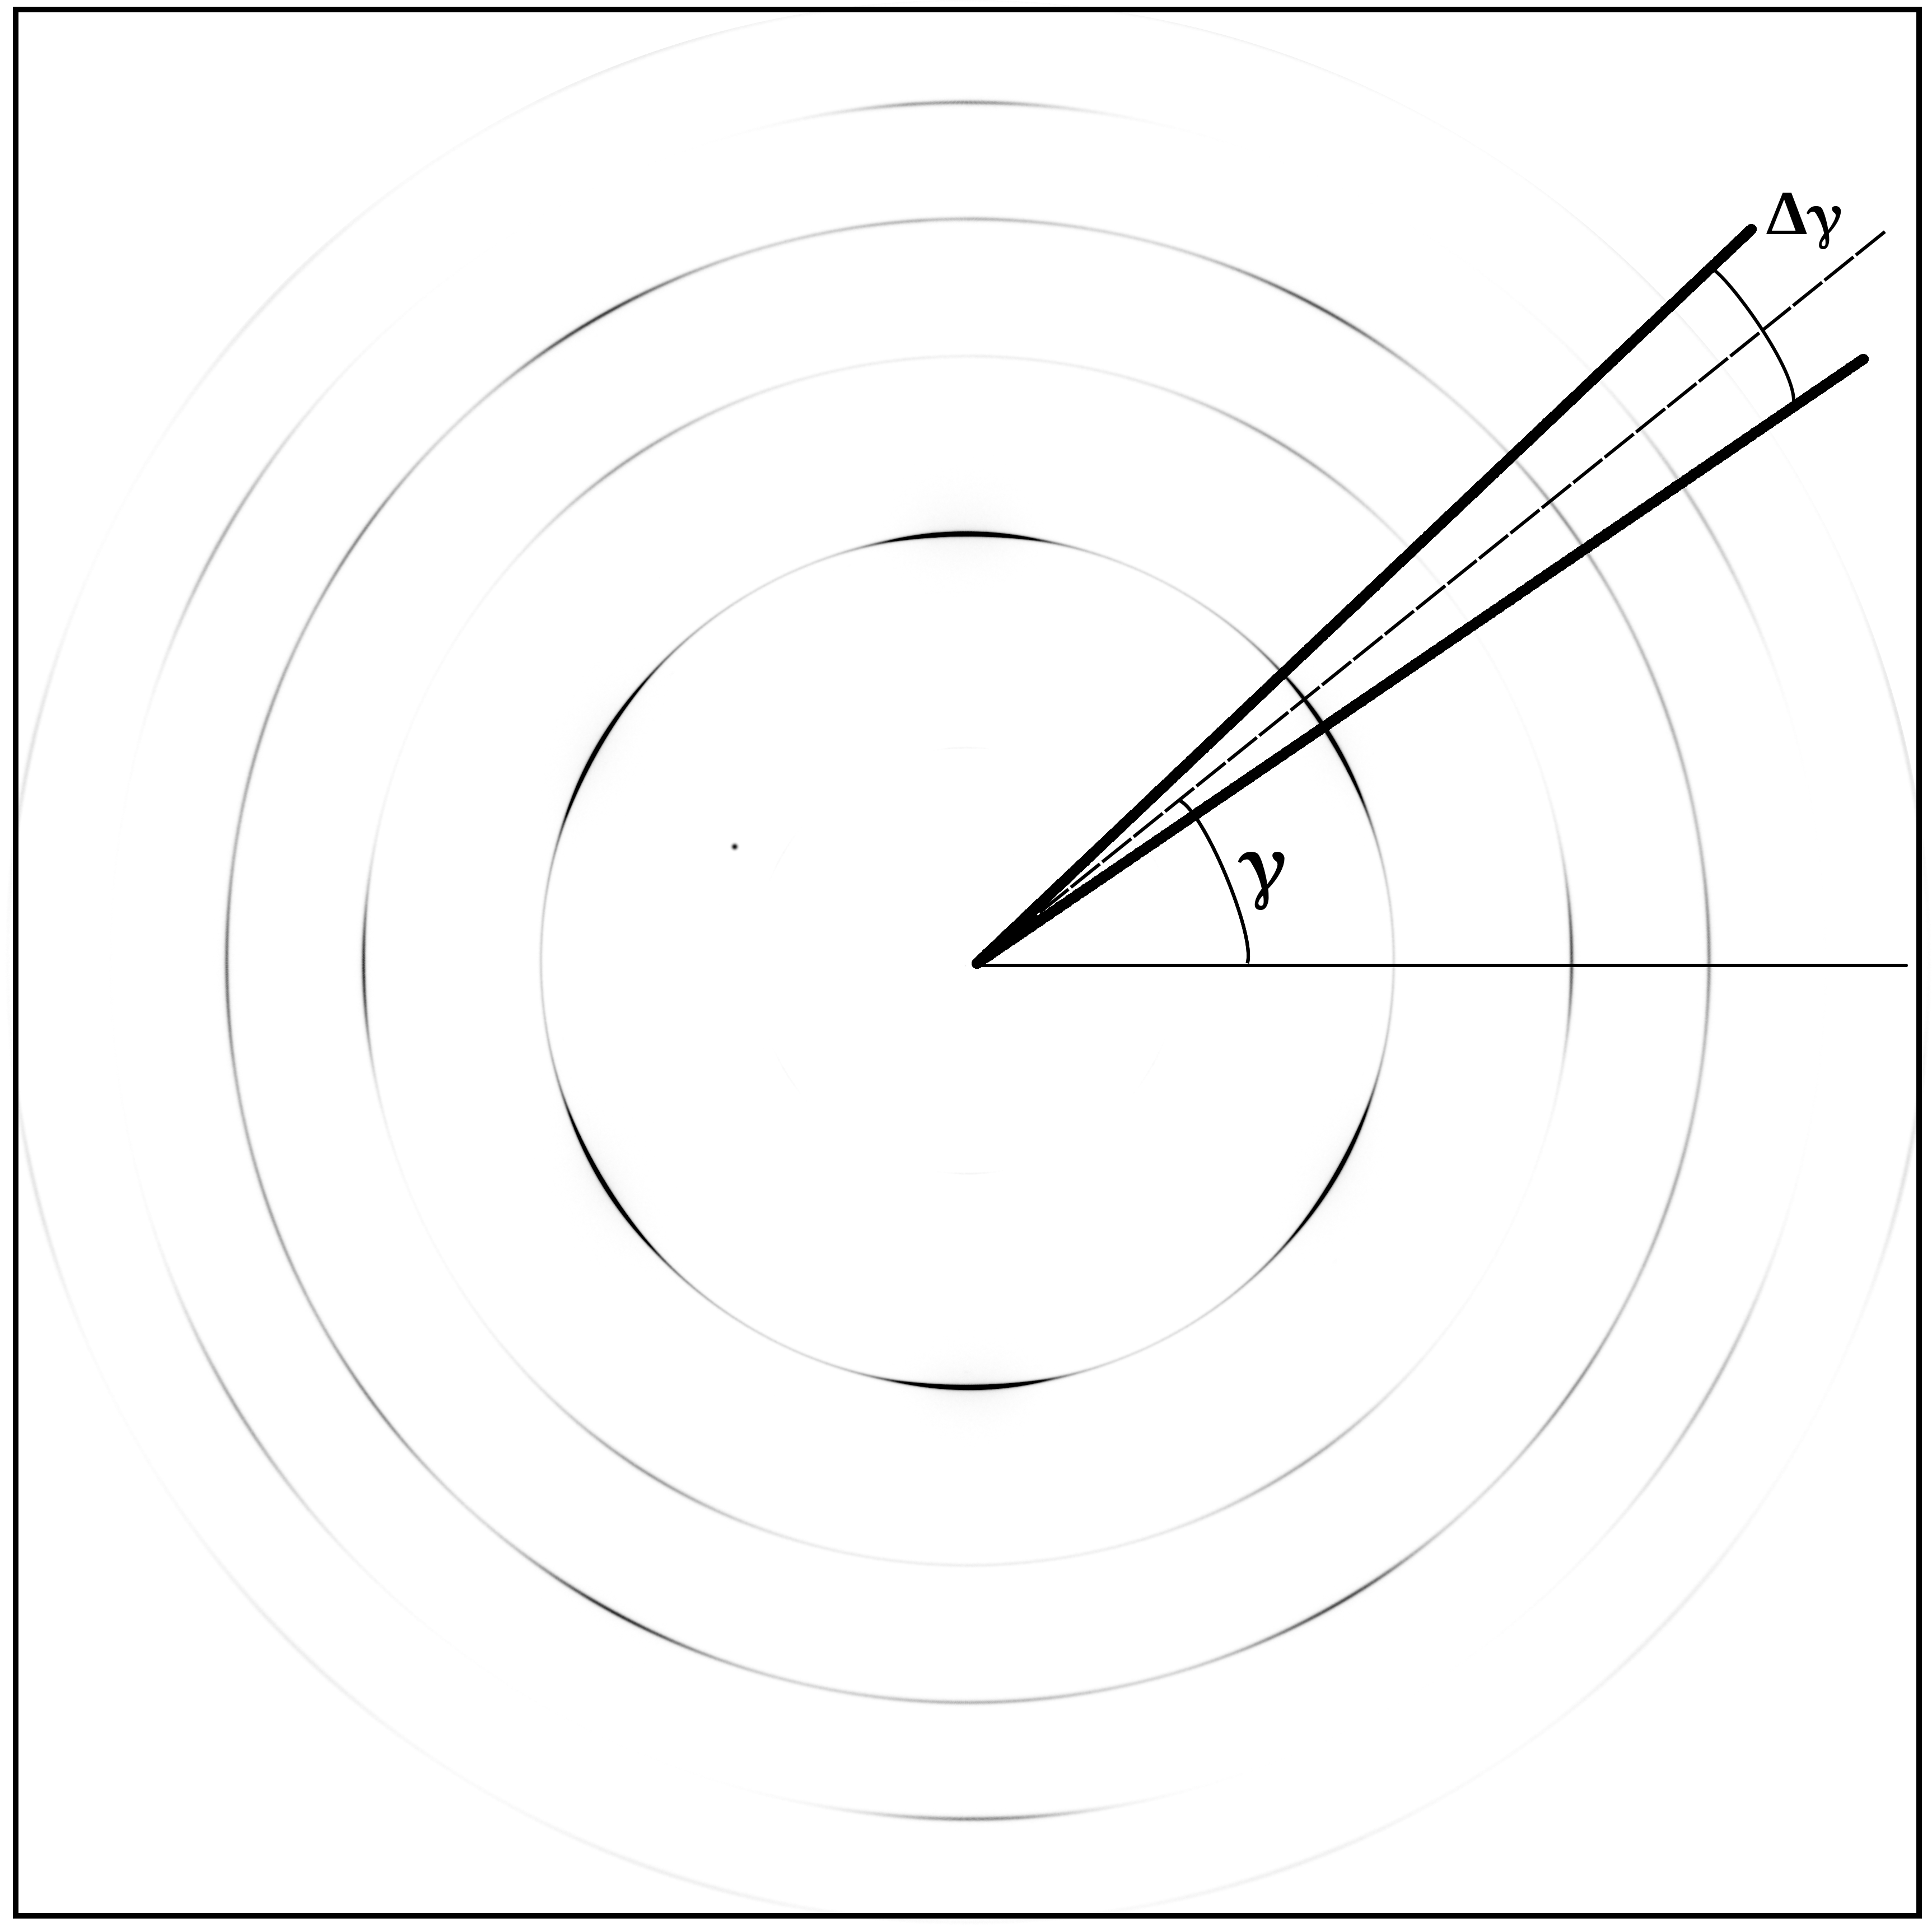
\includegraphics[width=0.5\textwidth]{Fit2D_2}
  \caption{Para convertir las imágenes grabadas en cada experimento de difracción se empleó el programa FIT2D, que permitió dividir a cada conjunto de anillos de Debye en 72 porciones de 5\,$^{\circ}$ cada una. El programa luego extraía la intensidad de promedio grabada dentro de cada porción y con esa información construía difractogramas que fueron luego empleado para realizar los ajustes.}
  \label{fig:fit2d}
\end{figure}

Una vez obtenidos todos los difractogramas, los mismos fueron tratados con un software de elaboración propia, tanto para aplicar el método de Langford como el CMWP.

Ambos softwares toman como dato de entrada todos los difractogramas obtenidos con FIT2D, además de otros archivos que deben ser escritos por el usuario, y que se encuentran ejemplificados en el apéndice \ref{CA:input}.

En el caso del programa que realiza el análisis de Langford se precisan tres archivos además de los datos extraídos de FIT2D.
El primero se denomina \hyperlink{datainfo}{data\_info\_1.ini} y contiene la información que indica dónde se guardarán los resultados y dónde se encuentran los archivos de entrada, así como su cantidad y los datos necesarios para realizar la conversión angular.
También la resolución en píxeles del detector y la distancia entre el detector y la muestra, datos necesarios para convertir las distancias sobre el detector a la variable 2$\theta$.
La opción \textit{Treshold} es un dato numérico que se emplea para determinar cuál es la intensidad mínima por encima del ruido de fondo que debe tener un pico para ser ajustado por el método de mínimo cuadrados. 
Como ajustar picos de baja intensidad puede llevar a alargar el tiempo que lleva procesar los datos, además de dar resultados poco confiables, no se recomienda colocar 0 como valor de umbral, mientras que un valor de 5 ha dado buenos resultados para las mediciones realizadas en esta tesis, como se puede ver en la Fig. \ref{fig:MinIntensity}

\begin{figure}[!htb]
  \centering
  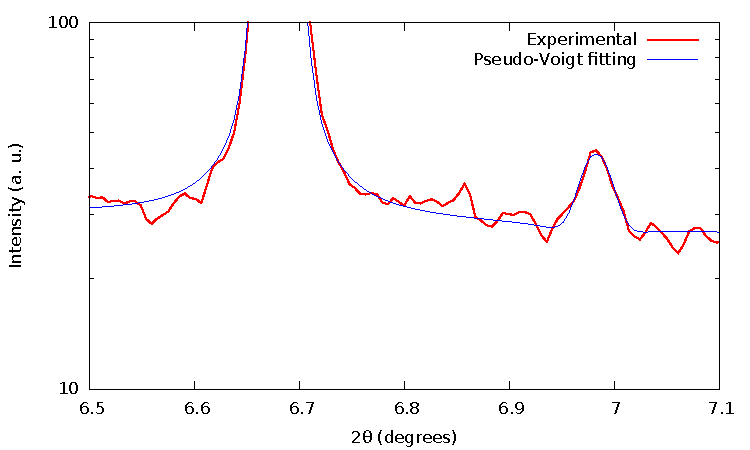
\includegraphics[width=0.8\textwidth]{Pico_minimo}
  \caption{La relación señal ruido mínima que permite distinguir y ajustar apropiadamente un pico del difractograma. El pico que se muestra tiene una intensidad integrada neta de 5 y como puede verse es ajustado razonablemente por una función pseudo-Voigt. Si el pico es más pequeño el error del ajuste se vuelve muy grande e incluso puede no converger.}
  \label{fig:MinIntensity}
\end{figure}

Las banderas \textit{Printpattern} y \textit{Correctwitdh} determinan si se van a imprimir los difractogramas extraídos junto con el mejor ajuste de cada uno, y si se van a realizar correcciones sobre el ancho de pico teniendo en cuenta el ancho de la muestra.
Esta es una característica experimental al momento de la escritura de la tesis, y debe emplearse con mucho cuidado.
Finalmente, también debe indicarse la cantidad de picos que se desean ajustar, junto con una coordenada aproximada de su centro (en 2$\theta$), los píxeles que definen inicio y final de cada pico, y dos píxeles que se determinarán el valor del ruido debajo de cada pico.

En el archivo \hypertarget{fitini}{\textit{fit\_ini\_2.ini}} debe indicarse nuevamente la cantidad de picos a ajustar, así como la cantidad de puntos de ruido que se ajustarán en la rutina de mínimos cuadrados.
La rutina de mínimos cuadrados minimiza la suma total de la diferencia entre las intensidades experimentales $I_{exp}$ y las intensidades teóricas $I_{teor}$ dadas por una suma de funciones pseudo-Voigt (Ec. \ref{eq:pseudovoigt}), una por cada pico, además de un ruido que se modela como una función lineal por partes, con $N_{ruido}$ partes, cantidad que es definida por el usuario:
\begin{equation}
  I_{teor} \ = \sum_{i=1}^{N_{picos}} \ pV_i (2\theta; \ I_{0i}, 2\theta_{B_i}, H_{gl}, \eta_{gl}, sH_i, s\eta_i) \ + \sum_{j=0}^{N_{ruido}} Bg(2\theta; \ I_{B_j}, I_{B_{j+1}})
  \label{eq:Iteor}
\end{equation}
\noindent
donde la función de ruido una función lineal dentro de un intervalo definido por $2\theta_j$ y $2\theta_{j+1}$ definido por el usuario y cero fuera de ese intervalo.
La función de ruido tiene intensidad $I_j$ en el punto $2\theta_j$ e intensidad $I_{j+1}$ en el punto $2\theta_{j+1}$, y las intensidades $I_j$ e $I_{j+1}$ son ajustadas dentro de la rutina de mínimos cuadrados.
De las funciones $pV(x)$, de las que hay una por pico, se ajusta su intensidad integrada $I_{0i}$, su centro $2\theta_{Bi}$ y su ancho y factor de mezcla.
El FWHM y el factor de mezcla de cada pico se generan a partir de un valor global (el mismo para todos los picos) y uno particular que se ajustan en pasos distintos del algoritmo de ajuste:

\begin{align}
  H_i & = H_{gll} \ + \ sH_i \nonumber \\
  \eta_i & =  \eta_{gl} \ + \ s\eta_i
  \label{eq:global}
\end{align}
\noindent
El motivo de esta separación es pura y exclusivamente por cuestiones de estabilidad numérica durante el ajuste, y no tiene una razón física detrás.

Todos los valores son ajustados por un rutina de mínimos cuadrados que emplea el algoritmo de Levenberg-Marquardt\cite{wiki:Levenberg} para minimizar el argumento de mínimos cuadrados:
\begin{equation}
  S(\mathbf{\chi}) \ = \ \sum_{i=1}^{N} (I^{exp}_i - I^{teor}_i(\mathbf{\chi}))^2
  \label{eq:argmin}
\end{equation}
\noindent
donde $\mathbf{\chi}$ es el conjunto de todos los parámetros que se varían para determinar la curva teórica que da el mejor ajuste a los datos experimentales.
Como el ajuste se realiza sobre cada difractograma en forma individual, $N$ indica la cantidad de mediciones que hay en un dado difractograma.

Una vez realizado el ajuste sobre todos los difractogramas, se toma la información de cada pico, el conjunto $(\theta_B, \ I_0, \ H, \ \eta)$ que tiene asociadas las coordenadas en el sistema de laboratorio $(\omega, \ \gamma, \ \theta_B)$ y se les asigna las coordenadas  $(\alpha, \ \beta)$ en el sistema de referencia del cristal, y con esos datos se construyen las figuras de polos y las figuras de polos generalizadas.
Antes de imprimir la salida de los archivos, el software substrae el ancho instrumental a partir de los valores que están presentes en el archivo \hyperlink{IRF}{\textit{IRF\_3.dat}}.
Las substracción de los datos se hace suponiendo que el ancho instrumental tiene una componente Gaussiana y una componente Lorentziana, y que ambas crecen con el ángulo $\theta$ siguiendo la ley de Caglioti\cite{Caglioti1958}:
\begin{align}
  \left[H_{ins}^{G}\right]^2 & =  U_G \ \tan^2(\theta) \ + \ V_G \ \tan(\theta) \ + \ W_G \nonumber \\
  H_{ins}^{L} & =  U_L \ \tan^2(\theta) \ + \ V_L \ \tan(\theta) \ + \ W_L
  \label{eq:caglioti}
\end{align}
\noindent
donde los parámetros $(U_i, V_i, W_i)$ deben ser especificados por el usuario.
En el archivo \textit{IRF\_3.dat} también deben especificarse los parámetros geométricos de la muestra para tener en cuenta la contribución del ancho de la muestra al ensanchamiento de los picos.

Los datos así obtenidos fueron procesados y graficados utilizando MTEX\cite{Hielscher2008}, un paquete de Matlab para el procesamiento de texturas.

El software que realiza el ajuste utilizando el método CMWP, tiene dos etapas básicamente: en la primera hace un ajuste al difractograma con una función como la mostrada en la Ec. \ref{eq:Iteor}, y siguiendo la metodología descripta anteriormente usa los resultados del ajuste para generar una serie de archivos auxiliares que se necesitan para la segunda etapa.
En la segunda etapa corre en forma automática el programa CMWP siguiendo una estrategia de ajuste determinada por el usuario.

Como la primera parte de este programa funciona con un objetivo similar al del programa anterior, el primer archivo de entrada, denominado \hyperlink{dinfoCMWP}{\textit{data\_info\_1.ini}} es casi igual al del programa anterior, con la diferencia de que al especificar la posición de los picos a ajustar se pide que se indique un número de fase que empieza en 0, ya que este es un dato necesario para el programa CMWP.

El segundo archivo se llama \hyperlink{fitstrategy}{\textit{fit\_strategy\_2.ini}} el usuario deber indicar los parámetros iniciales para el ajuste con pseudo-Voigts, como con el programa anterior, pero además deber indicar cuántos pasos de ajuste desea realizar con el programa CMWP, y cuáles son los coeficientes que va a ajustar en cada paso.
También debe indicar si desea que el CMWP haga un ajuste por fallas de apilamiento  y si desea que se ajuste independientemente la intensidad y posición de los picos.
En la práctica se ha visto que hacer un ajuste extra de intensidades alarga mucho el tiempo de cálculo del programa y no aporta valores finales muy diferentes a los que se obtienen cuando no se hace este ajuste.

Los siguientes tres archivos que debe generar el usuario son llamados archivos \textit{plantilla}, ya que estos archivos no suelen escribirse a mano, sino que son generados por el programa CMWP automáticamente, como ya se explicó en la Sec \ref{SS:CMWP}.

%\begin{figure}[!htb]
%  \centering
%  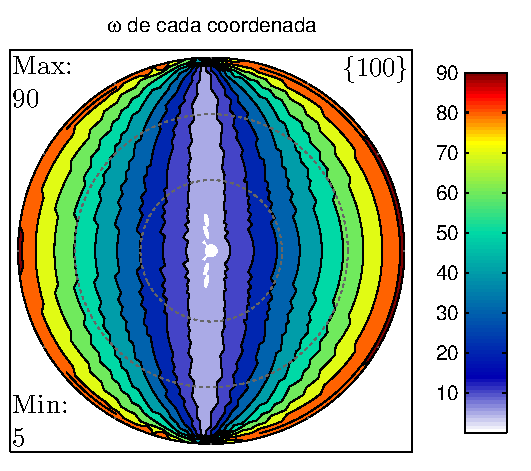
\includegraphics[width=0.8\textwidth]{Conv_PF_omega_contourf}
%  \caption{Relación entre las coordenadas angulares y las coordenadas de las figuras de polos.}
%  \label{fig:LabtoPF}
%\end{figure}

\iffalse
\subsection{Langford}\label{SS:MLgfrd}

\begin{figure}[!htb]
  \centering
  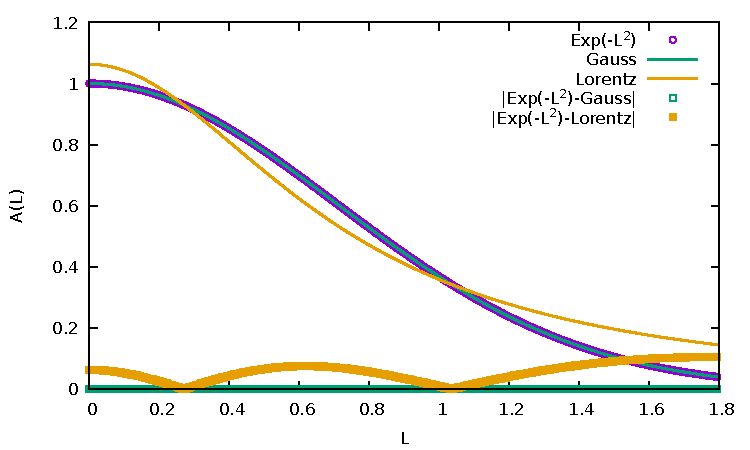
\includegraphics[width=0.8\textwidth]{GaussianStrain}
  \caption{Coeficientes de strain gaussiano y lorentziano.}
  \label{fig:GaussStrainn}
\end{figure}

\begin{figure}[!htb]
  \centering
  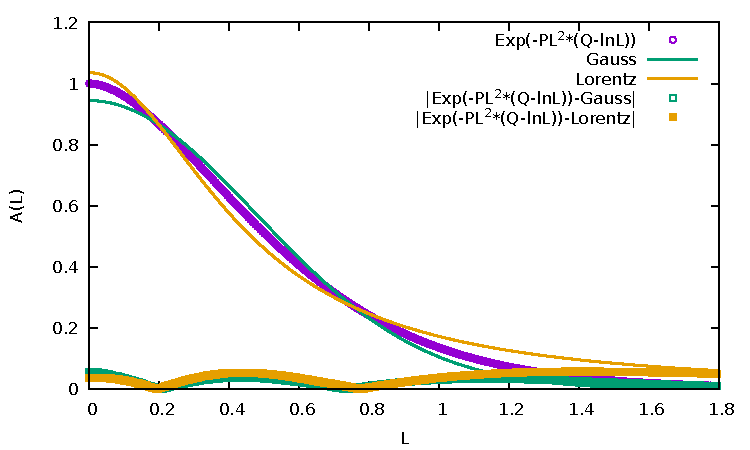
\includegraphics[width=0.8\textwidth]{RealStrain}
  \caption{Coeficientes de strain posta.}
  \label{fig:RealStrain}
\end{figure}

\begin{figure}[!htb]
  \centering
  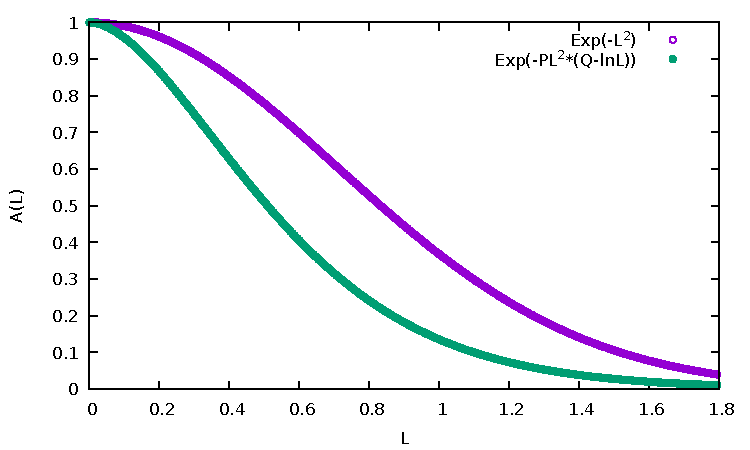
\includegraphics[width=0.8\textwidth]{Strain_Compare}
  \caption{Comparacion del gaussiano con el posta.}
  \label{fig:RealvsGauss}
\end{figure}

\newpage
\fi
\section{Mediciones de EBSD}\label{S:MatEBSD}
Los métodos de determinación de microestructura empleando difracción de rayos X tienen la ventaja de permitir estudiar propiedades volumétricas del material con una estadística más que razonable.
Sin embargo, dado que los estudios de ancho de pico son métodos indirectos que requieren la resolución de un problema matemáticamente mal planteado, en el transcurso de esta tesis fue necesario complementar los resultados obtenidos con mediciones de EBSD, que permite hacer una determinación más directa de ciertas características microestructurales, sobre todo aquellas que tienen que ver con la orientación de los cristales en el material.
Entre éstas se encuentran la textura cristalográfica, los tamaños de dominio y la deformación acumulada.

Las mediciones de EBSD fueron realizadas en el microscopio electrónico de barrido (SEM, por sus siglas en inglés) instalado en CCT Rosario - Laboratorio de Microscopía Electrónica de Barrido.
El mismo es un microscopio FEI Quanta 200E con cañón emisor de efecto de campo, detector de electrones secundarios y retrodispersados, con capacidad de trabajar en alto y bajo vacío y en condiciones ambientales (ESEM) y detector de EBSD (Ver Fig. \ref{fig:SEM}).
El software de adquisición empleado es TSL OIM Data Collection 5, para el análisi de los datos se emplearon los programas OIM TSL 7.3 y MTEX.

\begin{figure}[!htb]
  \centering
  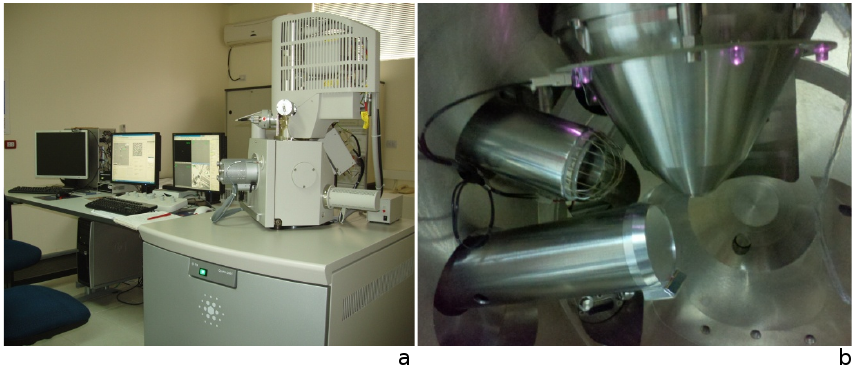
\includegraphics[width=\textwidth]{SEM}
  \caption{Fotografías del microscopio electrónico de barrido FEI Quanta 200E ubicado en el CCT Rosario - Laboratorio de Microscopía Electrónica de Barrido. (a) Vista externa del microscopio y computadoras para adquisición, análisis y soporte. (b) Imágen del interior del microscopio, donde se pueden apreciar el cañón emisor y los detectores.}
  \label{fig:SEM}
\end{figure}

La preparación de las muestras para este instrumento fue muy similar la utilizada para difracción de rayos X, pero el paso final de pulido electrolítico fue reemplazado por un pulido en sílica coloidal de 0.05\,$\mu$m; el motivo para este cambio es que el electropulido genera desniveles en la muestra donde hay alta energía almacenada (bordes de grano, dislocaciones, bordes de interfase), y como la muestra debe inclinarse 70$\circ$ para el análisis usando electrones retrodispersados estos desniveles distorsionan el desplazamiento de los electrones al interponerse en el camino del haz, y no se obtienen buenos patrones en estas zonas, dificultando la indexación.
El pulido con sílica coloidal, en cambio, consigue una superficie con mínimas rayas y relieves, por lo que resulta ideal para el análisis de EBSD.

Para determinar la textura del material con EBSD y poder compararla con la medida a través de XRD, es preciso hacer barridos de gran área para aumentar la estadística, lo que obliga a reducir la resolución del barrido para reducir el tiempo de barrido y de post-procesamiento.
Para los materiales estudiados, los barridos realizados para la determinación de textura se realizaron sobre áreas del orden de 600\,$\mu$m (RD) x 500\,$\mu$m (ND/TD) con una resolución de 0.4\,$\mu$m.
Se eligió que la dirección más larga del barrido sea siempre RD, ya que como la mayoría de los materiales estudiados fueron laminados, se esperaba que los granos fueran más largos en la dirección que laminado que en cualquiera de las direcciones perpendiculares.

El análisis de la anisotropía en la deformación acumulada y en el tamaño de grano se realizó sobre mapas con menor área y mayor resolución, ya que los detalles de la microestructura de los materiales deformados se pierden a resoluciones bajas.
Por ejemplo, si en un material deformado se espera tener granos de tamaño del orden de pocos micrones, o incluso de algunos nanómetros, si la resolución es de 0.4\,$\mu$m se cometer el error de asignar múltiples granos a un solo píxel.
Por lo tanto, los barridos realizados para obtener detalles de la microestructura se realizaron sobre áreas de 250\,$\mu$m (RD) x 80\,$\mu$m (ND/TD) con una resolución de 0.1\,$\mu$m.
Como se explicó en el párrafo anterior, fue preciso aumentar la longitud estudiada en la dirección de laminado de las muestras por la morfología que se esperaba observar en los granos de los materiales estudiados.

En esta tesis no se aplicaron métodos de “clean-up” para limpiar los datos ya que los puntos de los barridos con bajo índice de calidad corresponden a las zonas de alta deformación del material, y son precisamente estas zonas las que se intentan estudiar en esta tesis. 
Eso exigió un trabajo especial en obtener superficies adecuadas con la calidad necesaria para que la indexación sea la adecuada en una gran proporción de los puntos inspeccionados.

La determinación de la textura en las mediciones de EBSD es un proceso directo, ya que se mide la orientación de los cristales.
En el caso de MTEX, el cálculo de la ODF se hace a partir del desarrollo en serie de las llamadas funciones radialmente simétricas $\psi_L$:

\begin{equation}
  f(g) \ \sim \ \sum_{l=0}^{L} \sum_{k,k'=-l}^{l} \ \hat{f}(l, k, k') \ \psi_L(\omega(gg_i)) 
  \label{eq:ODFEBSD}
\end{equation}
\noindent
donde los coeficientes $\hat{f}$ del desarrollo \ref{eq:ODFEBSD} se calculan directamente a partir de las $N$ orientaciones $g_i$ medidas en el experimento de EBSD:
\begin{equation}
  \hat{f}(l, k, k') \ = \ \frac{1}{N} \ \frac{(l + 1/2)^{1/2}}{2 \pi} \sum_{i=1}^{N} \overline{D_l^{k k'} (g_i)}; \quad l \leq L, \ k, k' = -l, \cdots, l
  \label{eq:ODFcoef}
\end{equation}
\noindent
donde $D_l^{k k'}$ son los armónicos esféricos generalizados, y la barra denota conjugación compleja. Las funciones $\psi_L$ represetan orientaciones ideales en el espacio de orientaciones $SO(3)$ y son funciones de distribución que tienen su máximo cuando $g \ = \ g_i$ y decrecen monótonamente a medida que aumenta el ángulo $\omega$ entre $g$ y $g_i$.
Las funciones radialmente simétricas tienen asociado un ancho de de banda que se denota $\kappa$, que determina que tan intensa va a ser la textura alrededor de la orientación $g_i$.
A mayor $\kappa$, la distribución se vuelve más ancha y la textura menos intensa.

En teoría, el desarrollo \ref{eq:ODFEBSD} tiene infinitos términos, sin embargo por cuestiones de cómputo la serie se trunca en el $L$-ésimo término, que debe incrementarse para texturas muy intensas, es decir, en la medida que se quiera determinar una ODF muy intensa, el desarrollo en serie debe truncarse para $L$'s cada vez mayores, lo cual se logra reduciendo el parámetro $\kappa$ que condiciona el ancho de las funciones $\psi_L$.

La determinación de tamaño de grano en EBSD es conceptualmente distinta a los métodos análogos que se emplean en XRD o incluso en la metalografía tradicional.
Mientras que en XRD se obtiene una longitud promedio de las columnas cristalinas que difractan coherentemente en una dada dirección, en los análisis de EBSD el concepto de grano se define a partir de regiones cerradas que poseen una misorientación menor que cierto valor umbral definido por el usuario.
En general, y salvo que se especifique lo contrario, dos píxeles se considerarán en diferentes granos si su misorientación es mayor a 5\,$^{\circ}$, que es el criterio que se emplea normalmente en los análisis de EBSD.

La determinación de la deformación de la deformación acumulada en el material se hizo a partir del cálculo de las dislocaciones geométricamente necesarias (GND, por sus siglas en inglés).
El cálculo de las GND se hace a partir de calcular el tensor de Nye\cite{Nye1953}, que se calcula a partir de la curvatura de la red cristalina, que a su vez puede obtenerse a partir de medir la misorientación entre celdas vecinas\cite{Pantleon2008}.
La curvatura de la red cristalina se calcula midiendo la misorientación entre un dado pixel y sus vecinos en un dado mapa de EBSD, dejando afuera aquellos píxeles que pertenezcan a granos diferentes.
Debe notarse además que píxeles con una misorientación menor a los 0.5\,$^{\circ}$ tendrán una misorientación nula, ya que esa es la incerteza que se comete al medir misorientaciones con un microscopio como el empleado en este trabajo.
